\section{Mutation Analysis}

Attempting to improve a fuzzing effort is one way to find problems
with the effort; if you succeed, you found a weakness.  However, none
of the attempts exposed a serious problem.  Adding more fuzzers would
be \emph{good}, but was not obviously \emph{essential}.  Ensemble
fuzzing was not feasible, and swarm testing was, for practical
purposes, already performed by alternative means.  An alternative is
to directly look for holes in testing.  The Bitcoin Core fuzzing team
clearly was measuring and inspecting code coverage (see \url{https://marcofalke.github.io/btc_cov/}), so little value
would be added by inspecting traditional coverage alone.  Mutation
testing/analysis~\cite{MutationSurvey}, however, subsumes code coverage and adds extremely
valuable information on \emph{oracle power} in addition to mere
coverage~\cite{Discontents}.  This is perhaps especially valuable in fuzzing, where ``you
only see crashes'' is a persistent concern.

We used the universal mutator 

\noindent(\url{https://github.com/agroce/universalmutator})~\cite{regexpMut}, 
a mutation tool already used widely in the blockchain and smart contract
world, to mutate the Bitcoin and other popular cryptocurrencies core transaction verification code. 
Transaction verification is generally fairly well-covered, and obviously an extremely critical functionality for the
blockchain. 

Table \ref{tab:comparison} compares the mutation score, file coverage and project coverage over these transaction validation files. Mutation score represents the proportion
of mutants that were killed by the project's test suite divided by the total number of mutants. Higher mutation scores are usually indicative of better test suites, although this approach
of mutating a small subset of these projects does not entirely reflect overall test suite quality. File and project coverage metrics are both at the statement level.

\subsection{Mutation Testing Bitocin}

\begin{sloppypar}

For bitcoin, we ran universal mutator on {\tt tx\_verify.cpp} code. 
Figure~\ref{kills} shows an overview of the mutation analysis of the file.

\begin{figure}
\vspace{2mm}
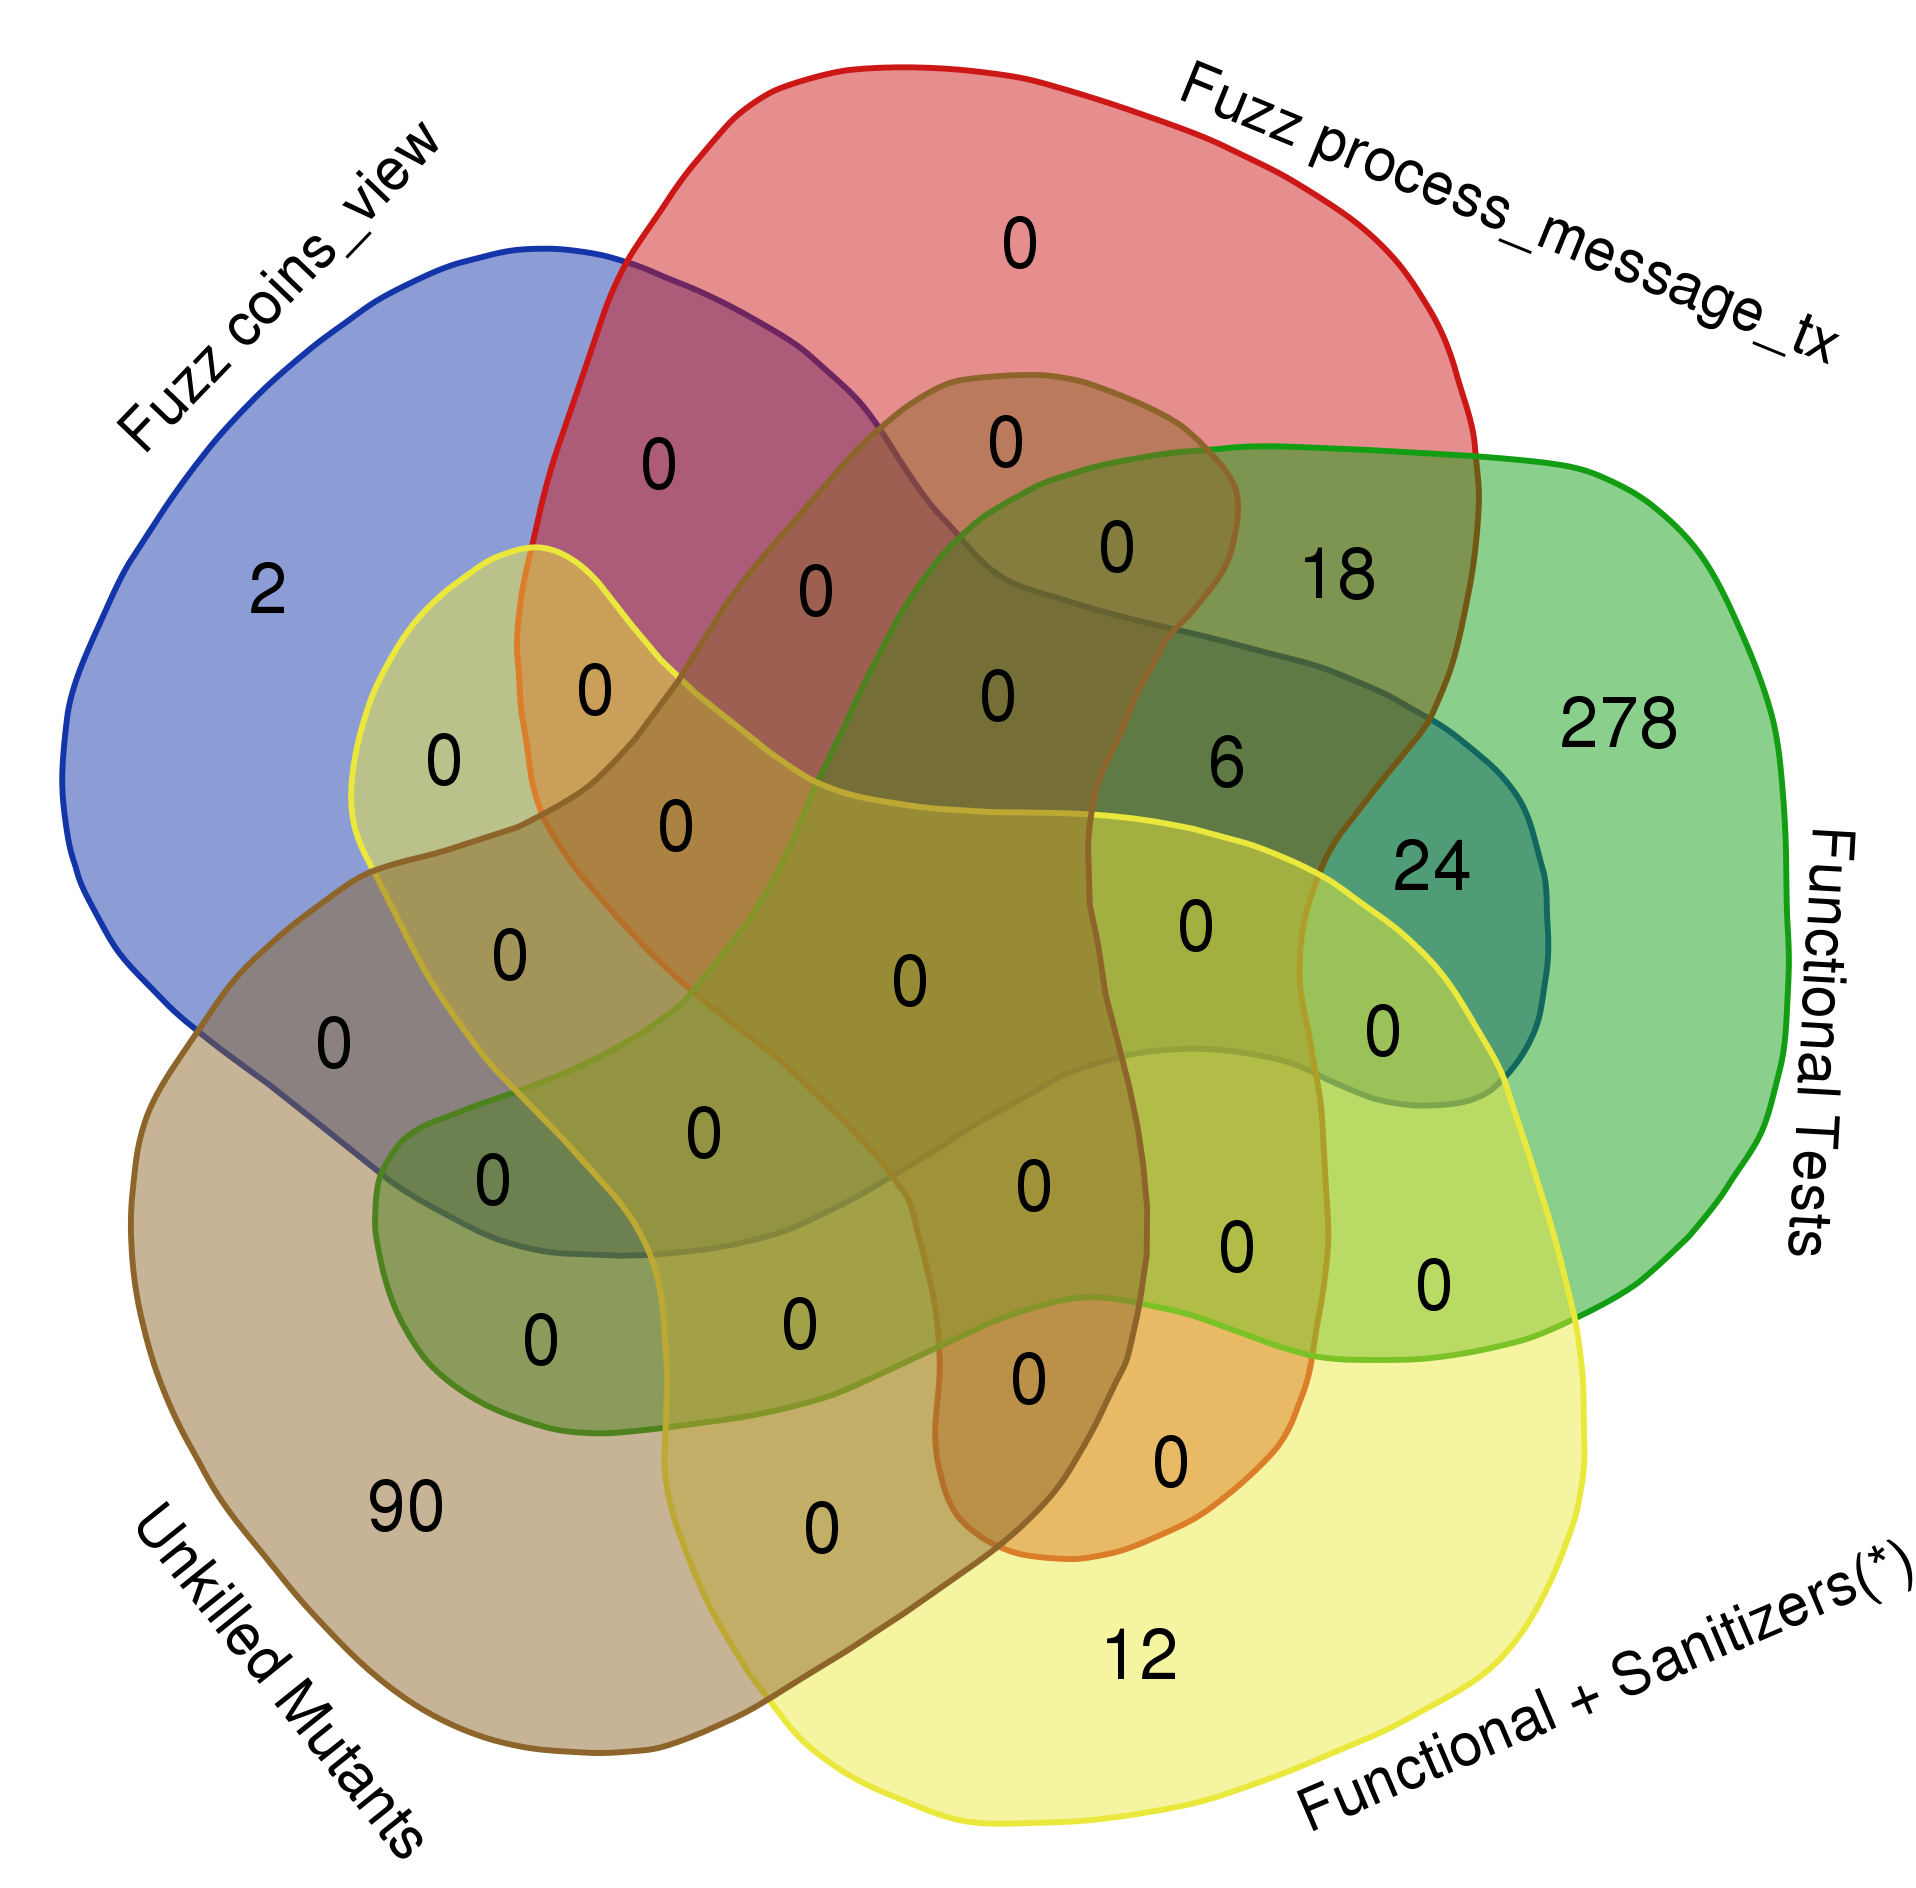
\includegraphics[width=0.9\columnwidth]{kill_pre_valgrind.png}
\caption{Mutation Kills for {\tt tx\_verify.cpp}}
\label{kills}
\end{figure}

The universal mutator generated 430 compiling mutants of the file.
Two fuzz targets performed interesting testing of the {\tt tx\_verify.cpp} code:
{\tt process\_message\_tx} and {\tt coins\_view}.  The code was also
tested by {\tt process\_message} and {\tt process\_messages} but the
relevant corpus entries were duplicated in {\tt process\_message\_tx}
(we verified these provided no additional mutant kills).  The fuzzing
applied was limited to five minutes of libFuzzer exploration based no
the full (and large) QA asset corpus for each harness, with all
sanitizers enabled.  The {\tt
  process\_message\_tx} target was able to detect 24 mutants, and the
{\tt coins\_view} harness was able to detect 32 mutants, for a total
of 50 mutants, not quite 12\% of all the generated mutants.  This is
not a bad result: fuzzing inherently has trouble detecting subtle,
non-crash-inducing, bugs in code, because writing a strong specification of
correct behavior that covers all the bizarre and pointless inputs
produced in fuzzing is often impractical, or would require a
specification nearly as complex as the code itself.  This is one
reason \emph{differential} fuzzing is promising: a reference
implementation is such a specification.  Bitcoin Core's cryptographic
elements are, in fact, differentially fuzzed
\url{https://github.com/bitcoin/bitcoin/pull/22704#issuecomment-898989809}.
\end{sloppypar}


A major purpose of fuzzing is, then, to address limits in more
traditional functional testing, where known inputs are paired with
expected behavior.  While functional or unit testing is very powerful,
the kinds of bugs found in vulnerabilities often involve the kind of
inputs that don't appear in ``normal'' unit/functional tests, as shown
by the success of fuzzing and security audits~\cite{FC20}.  The real
question, then, is how many mutants that survive Bitcoin Core's
extensive functional tests survive fuzzing.

The answer is: not too many.  The functional tests without sanitizers
enabled catch an additional 278 mutants.  Turning on sanitizers (which
is very expensive --- we \emph{only} ran it for mutants surviving all other
tests, as indicated by the zero overlap and the asterisk in Figure~\ref{kills}) catches an additional 12 mutants.  Only 90 of the
430 compiling mutants survive all tests, for an overall mutation score
of 79.07\%.  On the other hand, fuzzing only adds two mutant kills to
the functional testing.

Moreover, manual inspection of the surviving mutants showed that at
least 29 of these were clearly semantically equivalent to the
un-mutated code.  For instance, many mutants removed or weakened an
assertion; clearly this cannot ever be detected, since it can only
transform failing tests into passing tests.  The full, detailed list
of surviving mutants, prioritized by an FPF ranking~\cite{10.1145/2491956.2462173,Gonzalez85}, is
available here:
\url{https://github.com/agroce/bitcorpus/blob/master/mutation/prioritized_full_inspect.txt}.
Discussion with the Bitcoin Core team is ongoing as we write
(\url{https://github.com/bitcoin/bitcoin/issues/22690}), but thus far
none of the surviving mutants seem to expose serious testing
problems.  After manual pruning, the mutation score is 85.8\%, and
some of the remaining 61 mutants are likely also equivalent.  The
limitations of the fuzzing oracle are clear: fuzzing covers 98\% of
statements and72.6\% of branches as we write, but can kill fewer than
12\% of mutants.  The much greater killing power of the functional
tests obviously does not lie in the marginal 0.7 percentage points and 0.5
percentage points of statement and branch coverage obtained; it lies
in the ability to reject incorrect executions that do not crash or set
off a sanitizer alarm.

This raises the question:  why fuzz?  The coverage for high quality
(if imperfect) functional tests such as those for Bitcoin Core will
often be considerably
higher, and the oracle will almost always be \emph{much} more powerful.  The answer lies in the
fact that, even in the presence of such high quality tests, fuzzing
uncovers subtle bugs that functional tests designed by humans will
almost never detect,
e.g. \url{https://github.com/bitcoin/bitcoin/issues/22450}\footnote{Comments
  on this bug, such as ``Another win for fuzzing, oh wow.'' and
  ``Fuzzer rulez!'' show that the Bitcoin Core team has little doubt
  about the power of fuzzing.}.  Fuzzing is \emph{not} a replacement
for functional/unit tests; and functional/unit tests are not a
replacement for fuzzing.  In our mutation analysis, consider the two
mutants detected by {\tt coins\_view} fuzzing alone.  In the
traditional, score-based, view of mutation analysis, the {\tt
  coins\_view} fuzz harness would be seen as performing badly.  But it
detects 2 (hypothetical) bugs not detectable by other means; in the
real world, if one such bug is exploitable, detecting it may ``pay
for'' all the fuzzing effort, and there will seldom be just one such
bug (see
\url{https://github.com/bitcoin/bitcoin/issues?q=is\%3Aissue+fuzz+is\%3Aclosed+label\%3ABug}
for an approximate list of fuzzer-detected, fixed bugs in Bitcoin
Core).  If the ``good guys'' don't fuzz well, you can be sure the bad
guys will, for software protecting billions of dollars of assets.

\subsection{Comparison with Other Cryptocurrency Codebases}

\begin{table*}[ht!]
\vspace{2mm}
\centering
\begin{tabular}{llrccc}
\toprule
\bf \mr{2}{Project} & \bf \mr{2}{File Path} & \bf \mr{2}{LOC} & \mc{1}{c}{\bf Mutation} & \mc{1}{c}{\bf File}  & \mc{1}{c}{\bf Project} \\
\bf                 & \bf                   & \bf & \mc{1}{c}{\bf Score}    & \mc{1}{c}{\bf Coverage}               & \mc{1}{c}{\bf Coverage}  \\
\midrule
bitcoin & src/consensus/tx\_verify.cpp & 210 & 78.6\% & 98.7\% & 84.2\% \\
\cmidrule{2-6}
\mr{2}{go-ethereum} & core/block\_validator.go & 129 & 70.1\% & 81.0\% & 84.2\% \\
                    & signer/fourbyte/validation.go & 127 & 49.5\% & 60.0\% & 58.8\% \\
\cmidrule{2-6}
    \mr{3}{solana}   & perf/src/sigverify.rs & 1246 & ????\% & 74.48\% & \mr{3}{82.2\%} \\ 
    % & core/src/sigverify\_stage.rs &  296 & ????\% & 88.46\% & \mr{3}{82.2\%} \\  this seems to just call perf/src/sigverify
           & core/src/validator.rs & 2016 & -      & 73.29\% &        \\ % these are app.codecov.io/gh/solana-labs/solana @a6a4cfd numbers. grcov doesn't include tests, but reports coverage % as a total over lines including tests, so it's also not accurate. we'll just over approximate rather than underapproximate
           & core/src/tvu.rs       &  494 & -      & 63.12\% &       \\ 
\cmidrule{2-6}
  dogecoin & src/bitcoin-tx.cpp & 847 & 58.7\% & - & 70.1\% \\
\cmidrule{2-6}
  avalanchego & vms/platformvm/add\_subnet\_validator\_tx.go & 308 & 57.3\% & 81.0\% & 63.6\% \\
\cmidrule{2-6}
  stellar & src/historywork/VerifyTxResultsWork.cpp & 192 & 85.1\% & - & - \\
\cmidrule{2-6}
  go-algorand & ledger/eval.go & 1551 & 99.8\% & 86.0\% & 52.2\% \\
\cmidrule{2-6}
  cosmos-sdk & x/auth/ante/sigverify.go & 510 & 73.1\% & - &  - \\
\bottomrule
\end{tabular}

\caption{Code Coverage and Mutation Scores Across Popular Cryptocurrencies. Mutation score represents the proportion of mutants that were killed divided by the total number of mutants (higher is better). Coverage
metrics reported are at the statement level (proportion of statements covered in a file and in the entire project).}
\label{tab:comparison}
\end{table*}

\begin{figure}
\vspace{2mm}
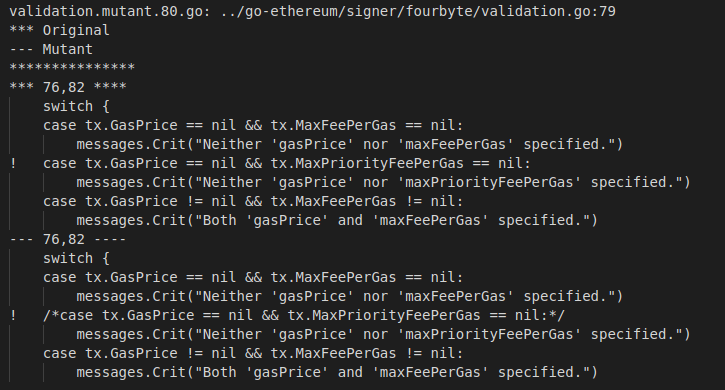
\includegraphics[width=0.9\columnwidth]{mutation-example.png}
\caption{Mutation Example for Ethereum Transaction Validation}
\label{fig:mutation}
\end{figure}

\begin{figure}
\vspace{2mm}
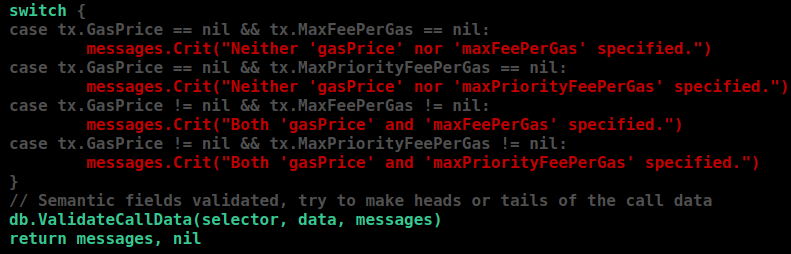
\includegraphics[width=0.9\columnwidth]{coverage-example.png}
\caption{Coverage Example for Ethereum Transaction Validation}
\label{fig:coverage}
\end{figure}

We also use mutation testing to (very loosely) compare Bitcoin Core's testing
with that for other popular cryptocurrencies. Again, we targeted
transaction validation logic, for the same reasons as given above. 
\newline
\newline
\noindent \textbf{Experiment Setup:} To select
our corpus, we examined the top 10 cryptocurrencies by market cap. We eliminate stable cryptocurrencies, such as USD coin,
because they do not have transaction validation logic analagous to bitcoin. For each project, we also run coverage collection
tools in order to compare code coverage. If a project does not build or have coverage, we also exclude it from our comparison.

In the end, the following projects failed to compile: Binance Coin, Polkadot, Chainlink and the following projects did not have
readily accessable coverage reports: Stellar.

We mutated files that are tested against interesting cryptocurrency properties, like signature verification, transaction and smart contract validity.
We found candidate files by searching each project for keywords transaction, verify, sign, and validate, manually inspected functions that perform corresponding operations,
and selected those files for mutation testing. The results of these experiments are displayed in Table \ref{tab:comparison}.
\newline
\newline
\noindent \textbf{Observations:} Interestingly, bitcoin seems to have among the highest coverage and mutation score out of any of the popular cryptocurrencies, with even forks of bitcoin, such as dogecoin having both lower
project coverage and mutation score. We suspect that this could be due to a variety of factors. Firstly, bitcoin reached out to the first author to investigate the quality of their test suite,
indicating that they emphasize and care about testing and quality. Secondly, other than go-ethereum, none of the cryptocurrencies besides bitcoin employed any kind of fuzzing, with bitcoin
employing continuous fuzzing through OSS fuzz to catch bugs. Finally, the bulk of our time was spent investigating bitcoin, making us most familiar with its codebase. There is a possibility
that we may have missed certain tests in other cryptocurrencies, as even in bitcoin the functional tests were not well-documented and difficult to find as a third party.

Furthermore, there does seem to be a correlation between coverage and mutation score, with files with high coverage typically killing the majority of the generated mutants. In cases with espcially
low coverage, such as ethereum's block and transaction validation code, many of the generated mutants were related to removing lines handling exceptional cases, which upon examination of the
file coverage were not covered. An example of this is shown in Figures \ref{fig:mutation}, \ref{fig:coverage}, with both the coverage report and an example mutant generated for ethereum. 
The lack of coverage of these exceptional cases across ethereum and many other low coverage files we examined, was something that surprised us, as we expected these files to have high coverage 
and test both happy and exceptional paths.
\newline
\newline
\noindent \textbf{Limitations:} One potential limitation of our analysis is the selection of files relating to transaction and block validation. While our heuristics and manual inspection did lead us to files that fulfilled these
properties, they were not comprehensive in finding all relevant files. Particularly in cryptocurrencies, such as ethereum, there is no one file that handles all transaction or block validation (a file analagous
to {\tt tx\_verify.cpp}  in bitcoin), but rather this logic is spread over dozens of different files. As a result, we are not able to make any definitive claims about the quality of these test suites, but rather
observations regarding mutation score and how good bitcoin's overall mutation score is. 

Furthermore, another limitation was that we spent more time was spent investigating bitcoin than any other cryptocurrency, meaning that there is a chance that we missed
some test that were not documented or easy to find in other cryptocurrencies.
